\documentclass{beamer}

\usetheme{Warsaw}

\usepackage[utf8]{inputenc}
\usepackage[T1]{fontenc}
\usepackage[frenchb]{babel}

\title{Présentation du Projet Ricochet Robot}
\author{Bamba Alassane
	\\Camara Mohamed
	\\Komara Mohamed Ba
	\\Salami Sodiki Olawale}
\date{\today}
\institute{Université de Caen Normandie}

\setbeamertemplate{navigation symbols}{}% pour enlever les symboles de navigation en bas de chaque page
\setbeamertemplate{footline}[frame number]%pour changer le pied de page par un affichage des numéros de slide

\begin{document}
	
	\maketitle
	
	%--------------------
	\begin{frame} 
		\frametitle{Plan}
		\tableofcontents
	\end{frame}
	%--------Section Introduction ------------
	\section{Introduction}
	
	\begin{frame}
		\frametitle{Introduction}
		
		L’unité d’enseignement de TPA (Travail Personnel Approfondi) a pour
		objectif de nous faire comprendre le concept de la programmation orientée
		objet, nous initier aux algorithmes d’intelligence artificielle et parfaire notre
		maitrise de java.
		
	\end{frame}
	
	%---------Sous Section Ricochet Robot --------------
	\subsection{Ricochet Robot}
	\begin{frame}
		\frametitle{Ricochet Robot}
		
		Ricochet Robots est un jeu de société créé par Alex Randolph et illustré par Franz 
		Vohwinkel , édité en 1999 par Hans Im Gluck / Tilsit.
		\\Le principe du jeu de société Ricochet Robots est de trouver en moins d’une
		minute la séquence de mouvement qui permettra à un robot donné (parmi
		quatre) d’atteindre un objectif désigné sur une case du plateau de jeu. 
		Cependant, les robots ne peuvent que se déplacer en ligne droite jusqu’à rencontrer
		un obstacle.
		
		\begin{figure}[htpb]
			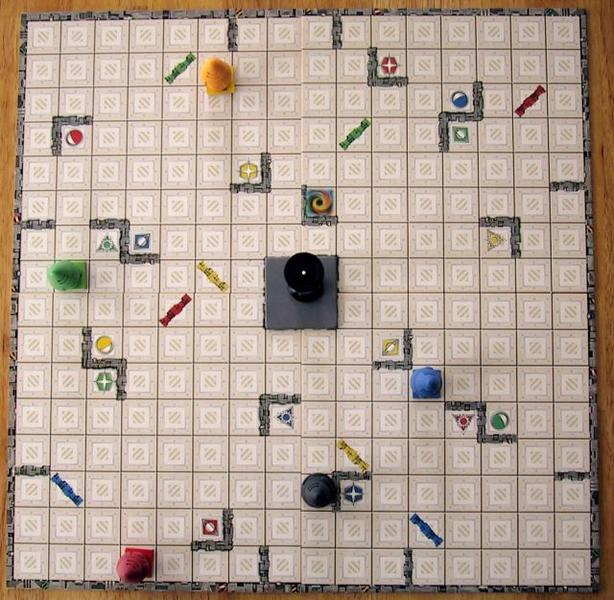
\includegraphics[scale=0.16]{./images/9.jpg}
		\end{figure}
		
	\end{frame}
	
	%---------Sous section Ojectif du projet --------------
	\subsection{Ojectif du projet}
	\begin{frame}
		\frametitle{Ojectif du projet}
		
		Le but de ce projet est de développer un programme permettant de trouver une solution optimale pour toute situation du jeu. 
		\\Dans un premier temps, il s'agira de développer le moteur du jeu (cf. règles) puis d'implanter un algorithme de résolution naïf, appelé A*. 
		\\Cependant, le problème est trop complexe pour être résolu dans de bonnes conditions. 
		\\Dans un second temps, il s'agira alors de proposer des méthodes d'optimisation de l'algorithme, par exemple en utilisant des tables de transposition. 
		\\Enfin, s'il reste du temps, il pourra être intéressant de réaliser une interface graphique permettant à un utilisateur de sélectionner un objectif. 
		
	\end{frame}
	
	%-------Section Organisation du projet-----------
	
	\section{Organisation du projet}
	
	\begin{frame}
		\frametitle{Organisation du projet}
		
		En ce qui concerne la répartition des taches, il est important de signaler que les tâches ont étés  départagées et nous avons travaillés régulièrement de façon grouper	afin de mieux comprendre individuellement chaque aspect du projet. 
		
	\end{frame}
	
	%---------Sous Section Répartition des taches--------------
	\subsection{Répartition des tachest}
	\begin{frame}
		\frametitle{Répartition des taches}
		
		Pour atteindre nos objectifs à temps et permettre à chacun d’entre nous de bien comprendre le projet, nous nous sommes séparés en binômes. Mohamed Ba Komara et Alassane Bamba se sont concentrés sur le monteur de jeu et l’algorithme A étoile, tandis que Mohamed Camara et Salami Sodiki Olawalé ont actés à la réalisation de l’interface graphique.
		Pour faciliter ce travail de groupe nous avons eu à nous retrouver souvent pour travailler avant le début du confinement et nous avons souvent utiliser une application appelée Team Viewer qui facilité le travail de groupe, mais depuis début des confinements nous travaillons essentiellement à travers cette application. 
		\end{frame}
	
	%---------Sous Section Architecture du programme--------------
	\subsection{Architecture du programme}
	\begin{frame}
		\frametitle{Architecture du programme}
		
		Pour ce projet nous avons opté pour une architecture MVC (Modèle Vue Contrôleur). Nous avons donc décomposé le projet en 5 packages :
		\\\textbf{PackageRR :} Il contient toutes les classes utilisées comme model de jeu à savoir la classe Case, Cible, Direction, Plateau, Robot etc voir figure 1\ref{figure1}.
		\\\textbf{PackageRR.ihm : } Dans ce package se trouve toutes les classes de la Vue.
		Images : Qui contient toutes les images utiliser dans ce projet 
		\\\textbf{PackageAEtoile : } Ce package contient les classes d’implémentation de l’algorithme de résolution naïf A*
		\\\textbf{PackageRR.execution:}  Ce package contient les classes d'execution du jeu.
		\\Avec cette architecture nous avons obtenus les diagrammes de classes suivants :
		
	\end{frame}
	
	\begin{frame}
		\begin{figure}[htpb]
			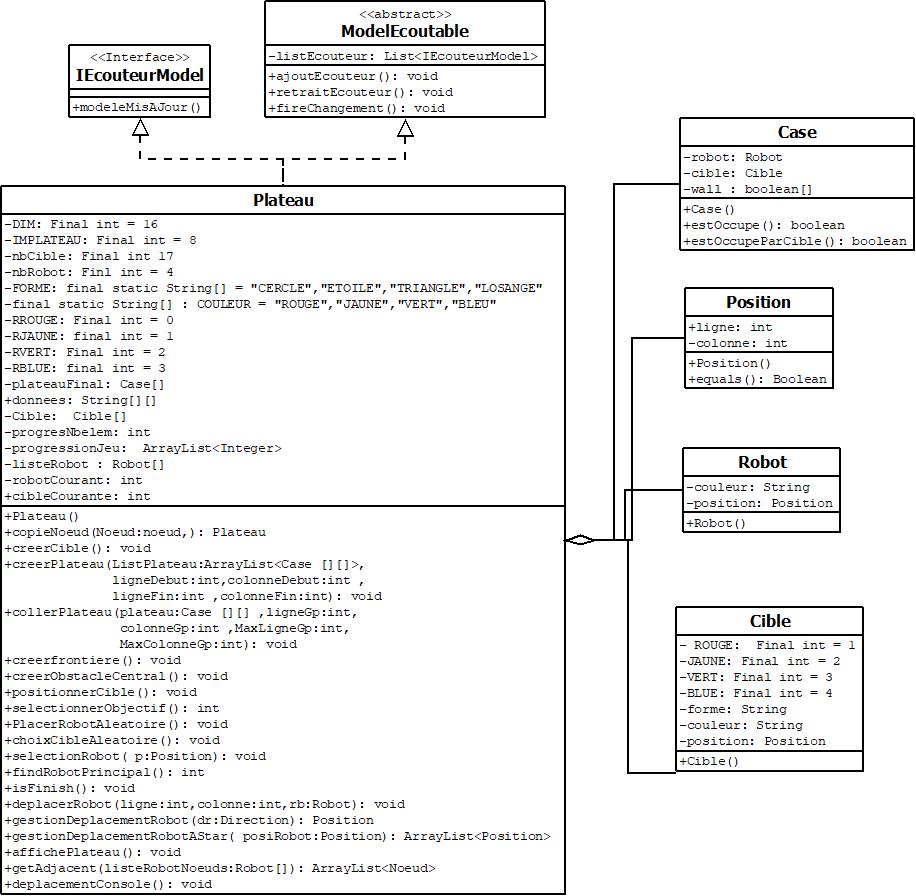
\includegraphics[scale=0.3]{./images/rr.jpg}
			\caption{Diagramme des classe du PackageRR \label{figure1} }
		\end{figure}
	\end{frame}

		\begin{frame}
		\begin{figure}[htpb]
			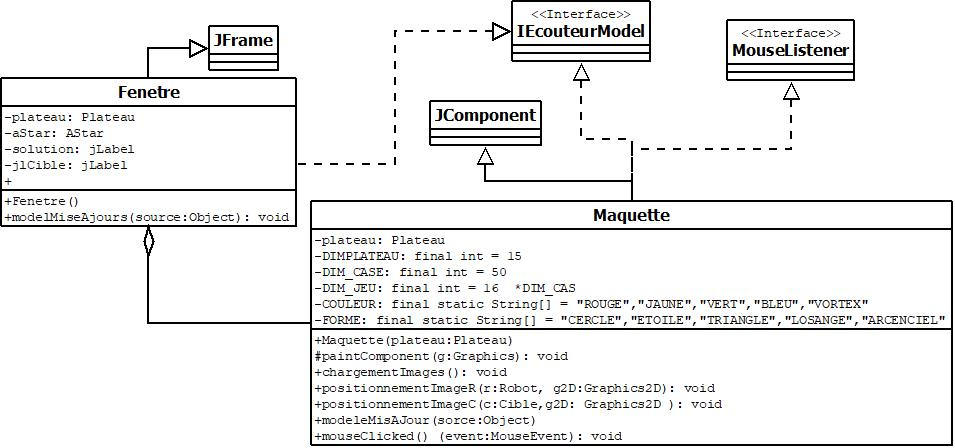
\includegraphics[scale=0.4]{./images/ihm.jpg}
			\caption{Diagramme des classe du PackageRR.ihm \label{figure1} }
		\end{figure}
	\end{frame}

			\begin{frame}
		\begin{figure}[htpb]
			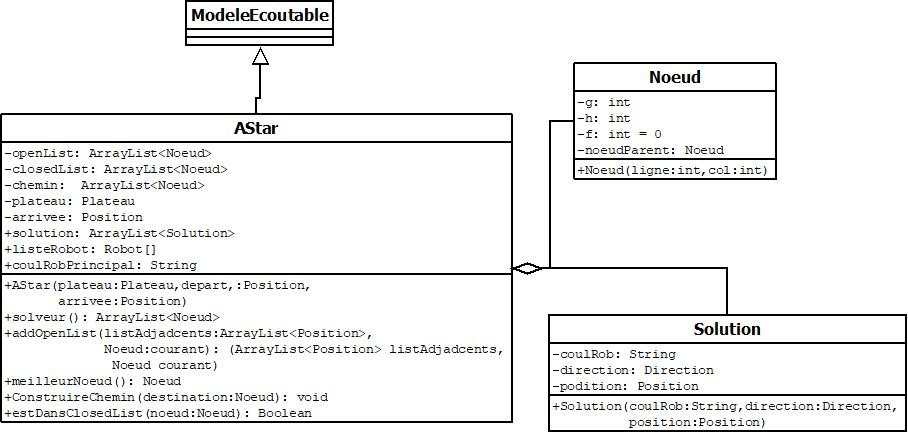
\includegraphics[scale=0.4]{./images/a.jpg}
			\caption{Diagramme des classe du PackageAEtoile \label{figure1} }
		\end{figure}
	\end{frame}

				\begin{frame}
		\begin{figure}[htpb]
			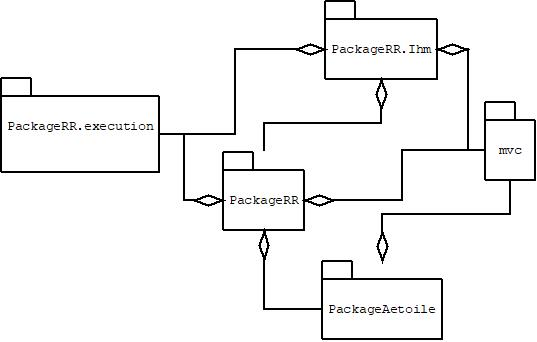
\includegraphics[scale=0.6]{./images/Package.jpg}
			\caption{Diagramme des Packages \label{figure1} }
		\end{figure}
	\end{frame}
	%-------Section Element technique-------------
	
	%---------Sous Section L’interface graphique--------------
	\subsection{L’interface graphique}
	\begin{frame}
		\frametitle{L’interface graphique}
		
		L'interface graphique répresente une partie nécéssaire pour la bonne visualisation du fonctionnement du jeu. Ainsi, nous avons utilisé des images qui nous ont permis de bien representer cette partie.
		
		L'interface est constitué d'un plateau sur le quel se trouve des robots, des cibles, des obstacles, des boutons de côntroles pour le deplacement des robots et pour l'execution de l'algorithme A* et enfin d'un label permettant la visualisation de la solution de l'Algorithme A*.
		
	\end{frame}
	\begin{frame}
		\frametitle{Affichage en console}
			\begin{figure}[htpb]
			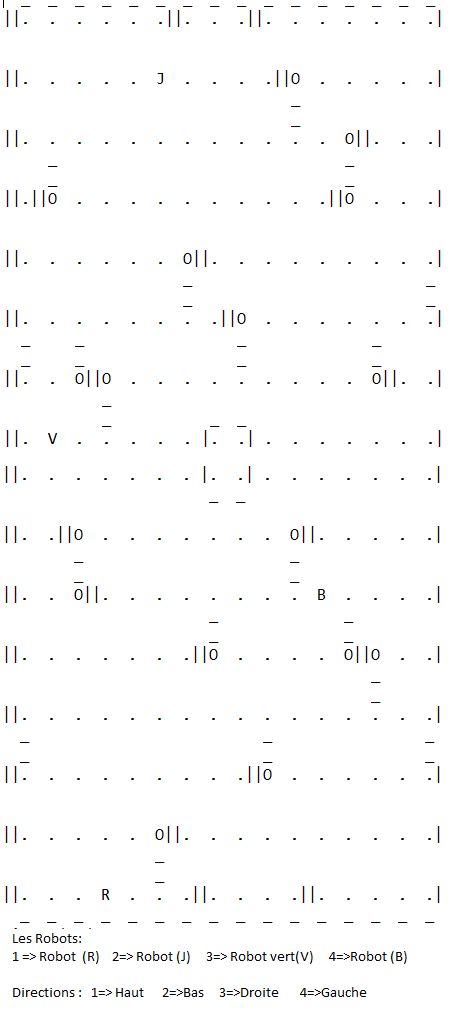
\includegraphics[scale=0.27]{./images/jeuConsole.png}
			\end{figure}
	\end{frame}

\end{frame}
\begin{frame}
\begin{figure}[htpb]
	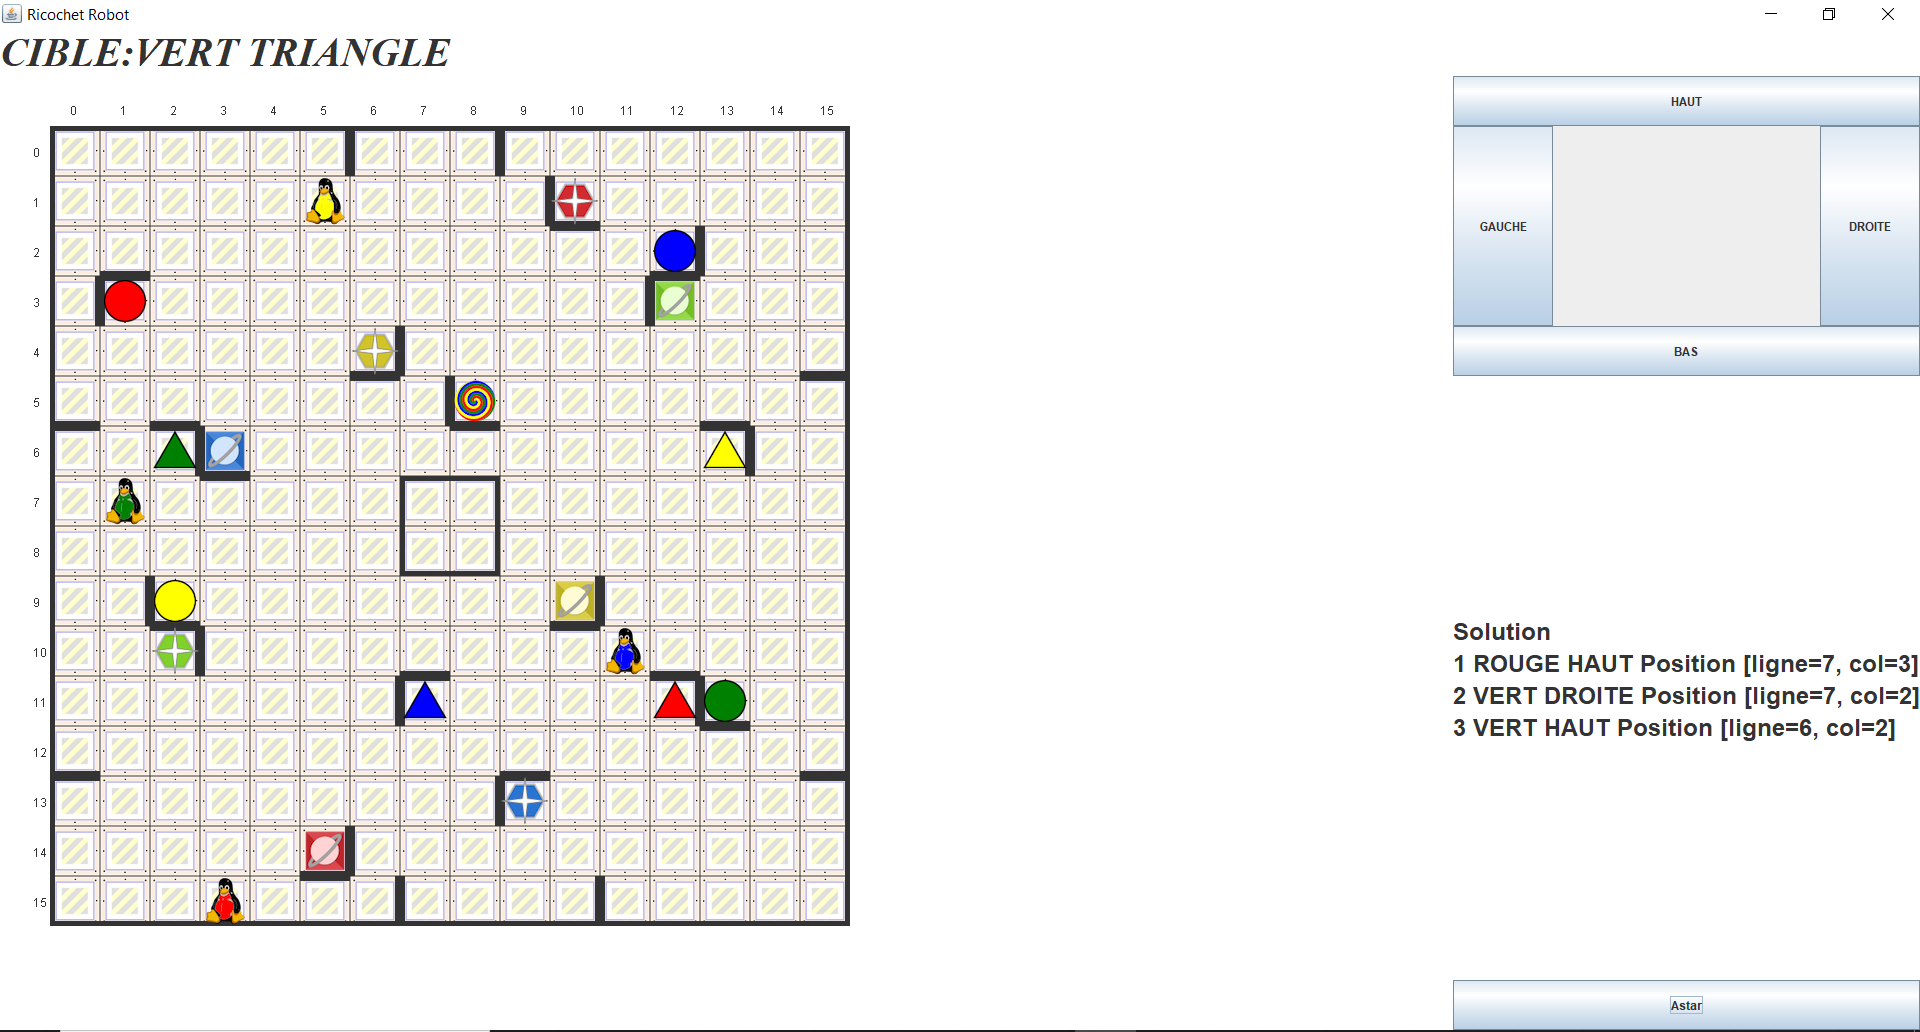
\includegraphics[scale=0.25]{./images/interface.png}
	\caption{Interface \label{figure1} }
	\end{figure}
\end{frame}
	
	%---------Sous Section Algorithme de résolution naïf A étoile (A*)--------------
	\subsection{Algorithme de résolution naïf A étoile (A*)}
	\begin{frame}
		\frametitle{Algorithme de résolution naïf A étoile (A*)}
		
			L’algorithme A* est un algorithme de recherche de chemin dans un graphe entre un nœud initial et un nœud final. Il utilise une évaluation heuristique sur chaque nœud pour estimer le meilleur chemin y passant, et visite ensuite les nœuds par ordre de cette évaluation heuristique.
		\\Dans notre cas un nœud est représenté par une liste contenant la position des 4 robots, de son nœud parent et de la valeur de sa fonction d’évaluation f.
		Cette fonction est calculée comme suit :f(n)=g(n)+h(n)
		— g(n) : représentant le coût du chemin entre le nœud de départ et le nœud n
		— h(n) : représentant le coût estimé entre le nœud n et le nœud d’arrivée ;c’est l’heuristique.
		G(n) est facile à être déterminé par contre h(n) est un petit peu plus compliqué et en plus la performance d’un algorithme A* dépend beaucoup de l’heuristique.
		Dans notre cas nous avons eu a implémenté 2 heuristiques :
			\end{frame}
		\begin{frame}
			\frametitle{Algorithme de résolution naïf A étoile (A*)}
		\\-  La distance à vol d’oiseau
		\\-  La distance de Manhattan
		Après plusieurs tests nous avons finalement fini par pencher pour celle de Manhattan qui mettait moins de temps que celle à vol d’oiseau.
		Fonctionnement : Le fonctionnement de l’algorithme est le suivant : Nous devons tout d’abord disposer de 2 listes : OpenList et closedList.
		Openlist : contient les nœuds qui n’ont pas encore été explorés
		ClosedList : contient les nœuds déjà explorés.
		Au début de l’algorithme, on considère le nœud initial comme étant la représentation du plateau de jeu à résoudre.
		\\-Ensuite On récupère tous les adjacents ce nœud. (16 adjacents avec la configuration actuelle)
		\		\-On ajoute tous ces adjacents dans l’openList du coup le nœud initial est ajouté à la closedList
		\\-Ensuite On récupère le meilleur nœud dans l’openList; c’est-à-dire celui qui a la plus petite valeur de f(n) et on  le 
	\end{frame}
\begin{frame}
	\frametitle{Algorithme de résolution naïf A étoile (A*)}
		supprime de cette liste pour l’ajouter dans la closedList.
		Donc tous les adjacents de ce nœud seront  à leur tour ainsi étudiés :
		\\ 1-  vérifier l’existence du nœud dans la closedList
		\\2-  S’il n’y existe pas on l’ajoute dans l’openList
		\\ 3-  Dans le cas contraire ,il y  existe donc on passe au nœud suivant ; cela voudrait dire qu’il a déjà été étudié.
		En gros on répète ces itérations successives jusqu’à atteindre un nœud où la position du robot principal sera identique à celle de la cible choisie ou jusqu’à vider l’openList.
		Une fois la solution obtenue on utilise la méthode construireChemin(courant) qui va parcourir la closedList de façon à reconstruire le chemin qui aboutit à la solution.  
		
		
	\end{frame}
	
	\begin{frame}
		\begin{figure}[htpb]
			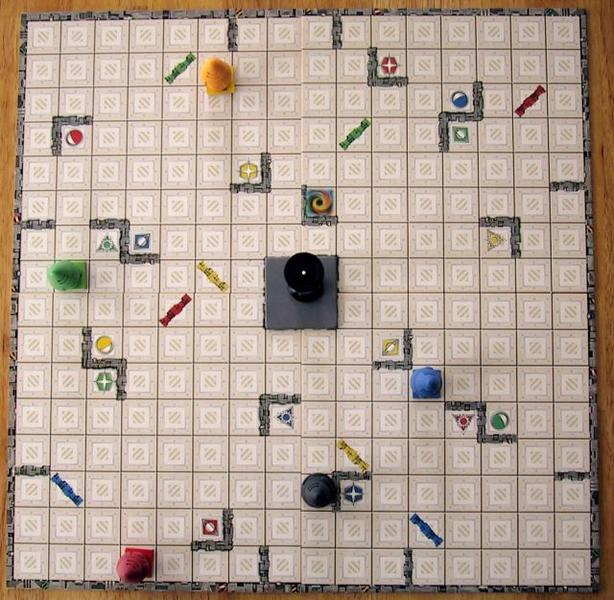
\includegraphics[scale=0.16]{./images/9.jpg}
			\caption{Diagramme des classe du PackageRR \label{figure1} }
		\end{figure}
	\end{frame}
	
	%------------Section Expérimentations et usages-------------
	\section{Expérimentations et usages}
	\begin{frame}
		\\\textbf{ Expérimentations }
		Après la réalisation du projet nous avions effectué de nombreux tests en ce qui concerne le fonctionnement du jeu et aussi l'utilisation de l'Algorithme A*.
		Au cours des différents tests effectués, nous avons constaté un temps de reponse plus ou moins long de l'algorithme A*.
		\\textbf{ Usages }
		\\\textbf{ Les robots:} Ils sont générés aléatoirements sur le plateau.
		\begin{figure}[htpb]
			
\includegraphics[scale=1.0]{./images/robot-red.png}
			
\includegraphics[scale=1.0]{./images/robot-yellow.png}
			
\includegraphics[scale=1.0]{./images/robot-green.png}
			
\includegraphics[scale=1.0]{./images/robot-blue.png}
			\caption{Robots \label{figure1} }
		\end{figure}
	\end{frame}

		\begin{frame}
		\\\textbf{ Le plateau:} Il sagit d'un plateau de seize lignes et colonnes  Composé de quatre petits plateaux générés aléatoirements. Sur chaque petit plateau sont fixés des obstacles permettant aux robots de ricocher. Aussi le plateau est encadré par des murs Haut, Bas, gauche et Droit.
		
		\begin{figure}[htpb]
			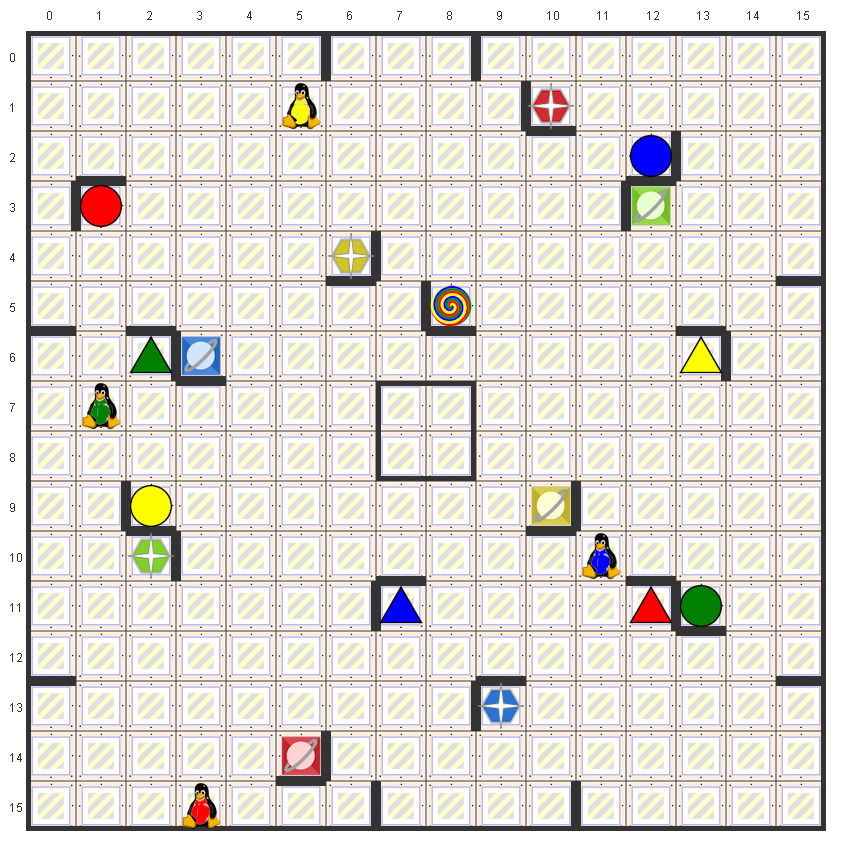
\includegraphics[scale=0.15]{./images/interfaceGr.png}
			\caption{Le plateau \label{figure1} }
		\end{figure}
		
	\end{frame}
	
	\begin{frame}
		\\\textbf{ Les boutons de controles:} ils permettent d'effectuer le deplacement des differents Robots. En effet après avoir sélection le robot à déplacé, il suffira de cliquer sur le bouton de direction souhaiteépour effectuer le déplacement.
		\begin{figure}[htpb]
			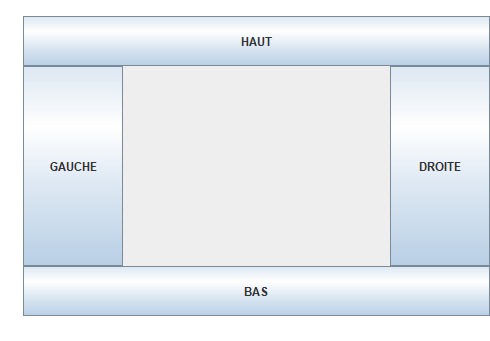
\includegraphics[scale=0.2]{./images/btnControl.png}
			\caption{Controls \label{figure1} }
		\end{figure}
		\\\textbf{ Le boutons Astar:} Après clic sur le bouton Astar, une solution sera afficher tout en  bas des boutons de control.
		
		\begin{figure}[htpb]
			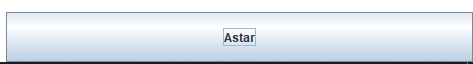
\includegraphics[scale=0.2]{./images/btnAstar.png}
			\caption{Boutons Astar \label{figure1} }
		\end{figure}
		
		
	\end{frame}
	%------------Section Conclusion -------------
	\section{Conclusion}
	
	
\begin{frame}
\frametitle{Conclusion}

	La réalisation de ce projet a été une occasion pour nous les membres de ce groupe d’apprendre encore plus le langage de programmation Java.
	Pendant ce projet, nous avons pu appliquer ce que nous avions appris dans les CM, les TP de ce semestre et ceux du semestre passé à savoir : la programmation orientée objet, la conception d’applications, les algorithmes récursifs et l’implémentation des algorithmes d’intelligence artificielle. 
	D'un point de vue humain, nous avons appris à mieux travailler en équipe, à communiquer, à bien organiser un travail d’équipe et le plus important à combler nos lacunes.  
	Nous avons également appris à travailler à distance en utilisant les outils de travail de groupe comme TEAM VIEWER et SVN.
\end{frame}
	
	%----Sous Section Objectifs remplis----------
	\subsection{Objectifs remplis}
	\begin{frame}
		\frametitle{Objectifs remplis}
		
		Dans ce projet, nous avions pour objectifs de réaliser le jeu Ricochet-Robots en implémentant toutes les règles du jeu dans une application JAVA et d’y implémenter l’algorithme de résolution naïf A*. Nous avons donc pu coder le moteur du jeu respectant toutes les règles du jeu, nous avons aussi réussi par faire une interface graphique afin que le jeu soit jouable pour un ou plusieurs joueurs, en jouant à l’aide des quatre buttons de déplacement, ainsi que l’affichage d'une solution possible en déplaçant les quatre robots avec l’algorithme de résolution naïf A*. 
		
	\end{frame}

		\begin{frame}
			\frametitle{Important}
				Pour visualiser la génération aléatoire des plateaux et des robots nous vous prions de bien vouloir décommenter les méthodes 
				suivantes: 
				\\Plateau ligne 90: rendre les plateaux aléatoires
				\\Plateau ligne 114: placer aleatoirement les robots
				\\Plateau ligne 123: rendre la première cible aléatoire
				\\NB: Elles ont été mises en commentaire pour minimiser le temps de réponse de l'Algorithme A* pour la première cible.
		\end{frame}
	
\end{document}
